\chapter{Test}
\label{chap:test}

\section{Test ``Analisi assistita''}
\noindent Per effettuare i test dell’estensione sono stati utilizzati alcuni siti realizzati per l’ultima edizione del concorso \textit{Accattivante Accessibile}.\
I test hanno preso in considerazione gli errori individuati da TV insieme a quelli segnalati dalla docente referente e sono stati messi a confronto con gli errori rilevati da \textit{SviluppAbile}.\
Infine, ho confrontato i risultati elaborando un resoconto per ciascun sito analizzato e, successivamente, ho applicato la metrica F1-score per ottenere un report oggettivo.

\subsection{F1-score} 
\noindent La F$_1$-score è una metrica utilizzata per valutare i modelli di classificazione, sia binari che multi‐classe. 
Essa combina in un unico valore la \textit{precision} (quanto le predizioni positive sono corrette) e il \textit{recall} (quanti casi positivi reali sono stati identificati), calcolandone la media armonica:

\[
F_{1} = 2 \cdot \frac{\text{Precision} \cdot \text{Recall}}{\text{Precision} + \text{Recall}}
\]

\noindent Questa formulazione assicura che il punteggio sia elevato solo quando entrambe le metriche hanno valori alti, penalizzando fortemente gli squilibri. 
La F$_1$-score risulta particolarmente utile in presenza di dati sbilanciati, poiché fornisce una valutazione più affidabile.

\subsection{Sito web: SudokuWorld}

\subsubsection{Total Validator}
\begin{figure}[H]
    \centering
    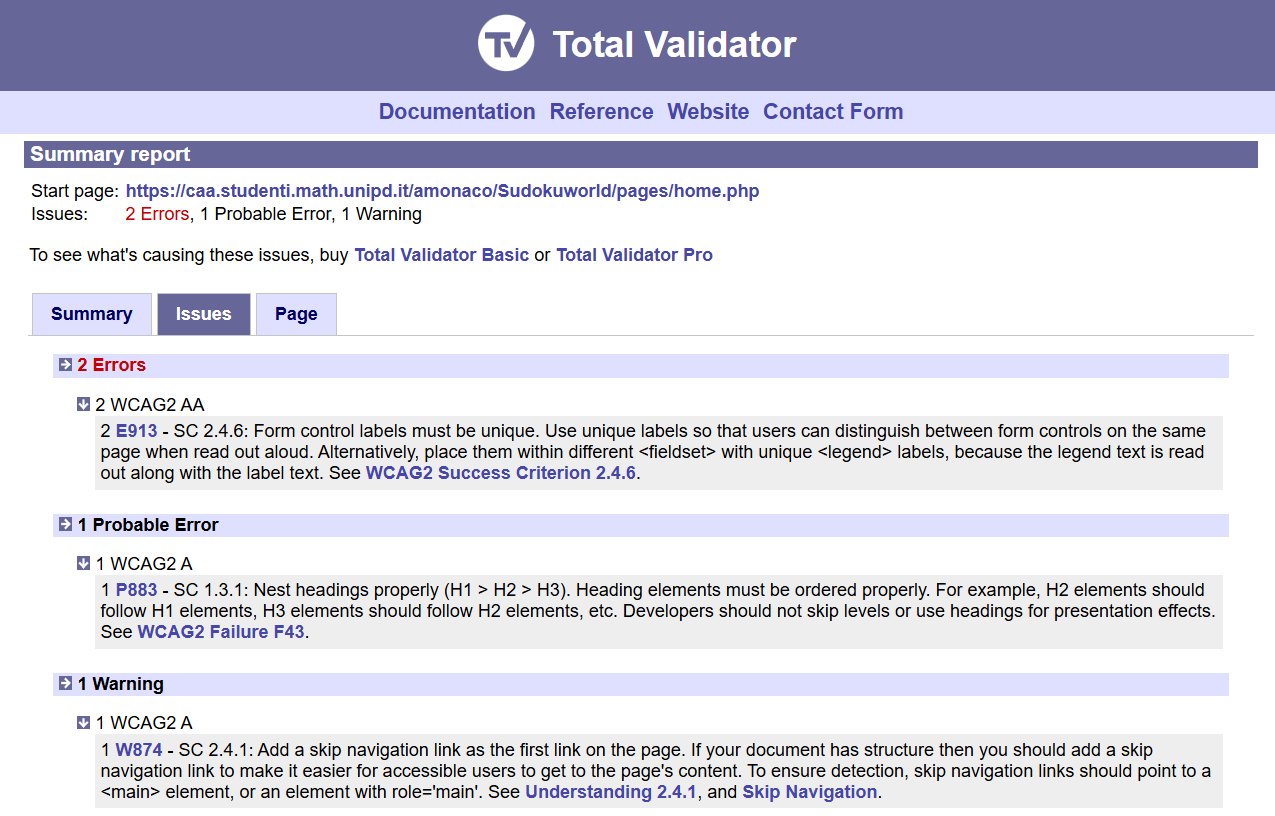
\includegraphics[width=0.7\linewidth, alt={Screenshot dell'analisi di Total Validator sul sito web SudokuWorld}]{img/TV_sudoku.png}
    \caption{Analisi di Total Validator sul sito web SudokuWorld}\label{fig:TV_sudoku}
\end{figure}

\noindent Come visibile nella figura \ref{fig:TV_sudoku} è possibile vedere che lo strumento \acrshort{tv} trova ben 15 errori di accessibilità.\\
Gli errori principali sono: 
\begin{itemize}
    \item E913 - SC 2.4.6: Le etichette dei controlli dei \glslink{formg}{form} devono essere univoche. Utilizzare etichette univoche consente agli utenti di distinguere i vari controlli presenti sulla stessa pagina quando vengono letti da uno screen reader. In alternativa, è possibile inserirli all’interno di diversi <fieldset> con <legend> univoci, poiché il testo del <legend> viene letto insieme all’etichetta del controllo. Vedi WCAG2 Success Criterion 2.4.6.
    \item P883 - SC 1.3.1: Nidificare correttamente le intestazioni (H1 > H2 > H3). Gli elementi di intestazione devono essere ordinati in modo gerarchico. Ad esempio, un elemento H2 dovrebbe seguire un H1, un H3 dovrebbe seguire un H2, e così via. Gli sviluppatori non devono saltare livelli né utilizzare le intestazioni solo per scopi di presentazione. Vedi WCAG2 Failure F43.
\end{itemize}

\subsubsection{Lighthouse}
\noindent Il report generato dallo strumento Lighthouse ha restituito un punteggio di 100/100 nella sezione Accessibility, indicando che, secondo le metriche automatiche adottate, non sono stati rilevati errori o problematiche di conformità (vedi figura \ref{fig:Lighthouse_sudoku}).
\begin{figure}[H]
    \centering
    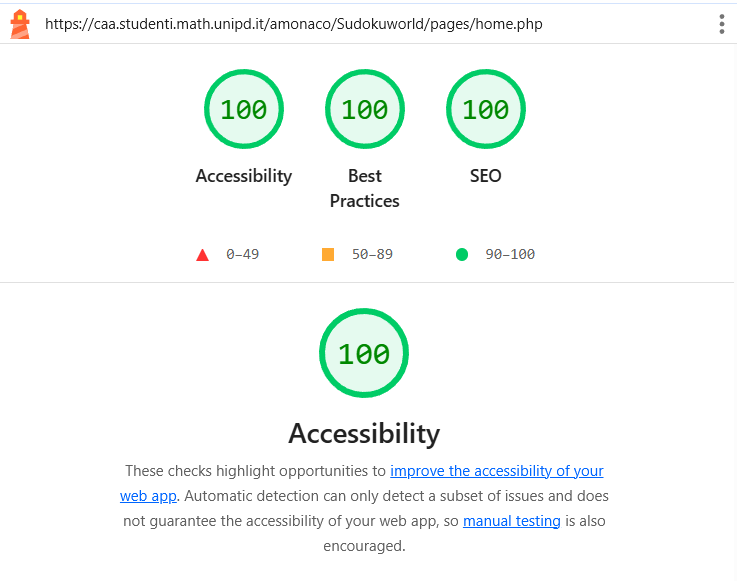
\includegraphics[width=0.6\linewidth, alt={Screenshot dell'analisi di Lighthouse sul sito web SudokuWorld}]{img/Lighthouse_sudoku.png}
    \caption{Analisi di Lighthouse sul sito web SudokuWorld}\label{fig:Lighthouse_sudoku}
\end{figure}

\subsubsection{SviluppAbile}
\noindent Di seguito vengono riportati i test effettuati con l'estensione \textit{SviluppAbile}. \newline
\\ \vspace{-0.5cm}
\noindent(pagina home.php)
\subsubsection*{\texttt{Il mio codice HTML rispetta le linee guida WCAG?}}
\begin{adjustwidth}{1cm}{1cm}
\noindent {\footnotesize Il tuo codice HTML sembra essere in parte conforme alle linee guida WCAG (Web Content Accessibility Guidelines), ma potrebbe migliorare ulteriormente per garantire una maggiore accessibilità. Alcune aree che richiedono ulteriore attenzione includono:\\
- L'attributo `aria-label` non è utilizzato in modo coerente nei controlli di navigazione.\\
- Le etichette dei pulsanti "Cerca" e "Profilo" potrebbero essere più descrittive.\\
Tuttavia, il tuo codice include molti elementi positivi come l'utilizzo di `alt` per immagini, la presenza di un titolo (`<title>`) e di metatag di descrizione (`<meta name="description">`). Questi sono passaggi fondamentali per migliorare la comprensione del contenuto da parte dei motori di ricerca e degli assistenti.\\
Per garantire una maggiore accessibilità, considera di applicare ulteriormente le linee guida WCAG 2.1, che offrono standard e raccomandazioni per creare esperienze web più inclusive.\\
La pagina non rispetta la norma W3C WCAG 2.1 che richiede di nidificare correttamente le intestazioni. Non sono presenti elementi HTML con attributo "h1", mentre ci sono intestazioni con grado inferiore.\\
La situazione descritta viola la regola WCAG 1.3.1, che richiede la corretta gerarchia di intestazioni (H1 > H2 > H3). In questo caso, l'h2 non è diretto al figlio dell'H1.\\
Vi è inoltre la presenza di due etichette (label) con il valore "Cerca" all'interno della stessa pagina HTML, ma con attributi id diversi ("searched-product" e "for"). Secondo la specifica SC 2.4.6, le etichette dei form control devono essere uniche.
}
\end{adjustwidth}

\subsubsection*{\texttt{Vi sono errori riguardanti i link?}}
\begin{adjustwidth}{1cm}{1cm}
\noindent {\footnotesize Il codice HTML contiene due carousel circolari:\\
1.  Il primo è definito come "specialProductsCarousel" e si trova nella sezione `<main>`.\\
2.  Il secondo è chiamato "bestSellersCarousel" ed è anch'esso presente all'interno della stessa sezione.\\
Quanto ai controlli sui link visitati, non sono implementati controlli specifici per la traccia dei link visitati sul sito web.
} \\
\end{adjustwidth}

\noindent(pagina sudoku.php)
\vspace{-0.5cm}
\subsubsection*{\texttt{Il mio codice HTML rispetta le linee guida WCAG?}} 
\begin{adjustwidth}{1cm}{1cm}
\noindent {\footnotesize Il tuo codice HTML non rispetta pienamente le linee guida WCAG (Web Content Accessibility Guidelines) per diverse ragioni:\\
1.  **La navigazione è troppo complessa**: la barra di navigazione contiene molti elementi e link, potrebbe essere difficile per gli utenti disabili utilizzare l'interfaccia.\\
2.  **L'accessibilità dei form è insufficiente**: non sono presenti attributi accessibili per i campi di input e submit, rendendo la navigazione dei form difficoltosa per gli utenti che usano dispositivi di assistenza.\\
3.  **La lettura dei testi in basso risulta difficile**: alcuni elementi come il timer sono troppo piccoli per essere letti facilmente dagli schermi con alto contrasto o da dispositivi di assistenza.\\
4.  **Non ci sono alternative al linguaggio naturale**: le immagini contengono solo icone e simboli, che potrebbero non essere compresi da utenti analfabetici.\\
\\Aggiungere attributi accessibili ai campi input e submit:\\
*   Modifica il codice HTML come segue:\\
    \texttt{<form class="d-flex align-items-center my-2 my-lg-0 ms-auto" \\ action="/amonaco/Sudokuworld/pages/search.php" method="GET"> 
    \begin{adjustwidth}{1cm}{}  <label for="searched-product" class="visually-hidden">Cerca</label>\end{adjustwidth}
    \begin{adjustwidth}{1cm}{} 
        <input class="form-control me-2" type="search" name="searched-product" id="searched-product" placeholder="Cerca" value="" aria-label="Search" />
    \end{adjustwidth}
    \begin{adjustwidth}{1cm}{} 
        <button class="btn btn-outline-success" type="submit" \textbf{aria-label="Submit the form"}>Cerca</button>
    \end{adjustwidth}
    </form>}\\
\\Aggiungere tag alt alle immagini: assicurati di aggiungere il contenuto alternativo per ogni immagine.\\
*   Modifica il codice HTML come segue:\\
    \texttt{<a class="nav-link" href="/amonaco/Sudokuworld/pages/sudoku.php">\\
    \indent <i class="bi bi-grid-3x3-gap-fill"></i>\\
    </a>}\\
\\Aggiungere tag aria: per fornire informazioni aggiuntive alle pagine web, puoi utilizzare gli attributi aria.\\
*   Modifica il codice HTML come segue:\\
    \texttt{<h1 class="container border border-black p-2 mb-4 rounded text-center" id="sudokuTitle" role="heading" aria-level="1">!! Sudoku !!</h1>}\\
\\Controlla l'accessibilità con strumenti di testing: prima della pubblicazione, assicurati di utilizzare strumenti come Lighthouse o WAVE per valutare la tua pagina web e risolvere eventuali problemi.\\
Ricorda che un sito web accessibile è più facile da utilizzare per tutti gli utenti, compresi quelli con disabilità.\\
\\
\texttt{DOMANDE SUGGERITE: \\"Quale è il criterio WCAG 2.1 che riguarda la navigazione con tastiera?"
\\"Come posso utilizzare gli strumenti di analisi del codice per identificare le aree dell'accessibilità da migliorare nel mio sito web HTML?"
}}
\end{adjustwidth}

\paragraph*{\texttt{"Come posso utilizzare gli strumenti di analisi del codice per \\ identificare le aree dell'accessibilità da migliorare nel mio sito web HTML?"}} 
\begin{adjustwidth}{1cm}{1cm}
\noindent {\footnotesize Per identificare le aree dell'accessibilità da migliorare nel tuo sito web HTML, puoi utilizzare gli strumenti di analisi come W3C Validator e Lighthouse. Il W3C Validator verifica la correttezza del codice HTML e fornisce suggerimenti per migliorare l'accessibilità. Lighthouse è uno strumento open-source che valuta l'accessibilità, le prestazioni e la sicurezza del tuo sito web.}
\end{adjustwidth}

\paragraph*{\texttt{"Come posso utilizzare le liste di controllo di WCAG (Web Content Accessibility Guidelines) per migliorare l'accessibilità nel mio sito web?"}} 
\begin{adjustwidth}{1cm}{1cm}
\noindent {\footnotesize Le Liste di Controllo (LC) di WCAG 2.1 forniscono un quadro dettagliato per valutare e migliorare l'accessibilità del tuo sito web.\\
Per iniziare, leggi attentamente le LC relative alle sezioni più rilevanti per il tuo sito:\\
* Guida per i fornitori di contenuti (G): informazioni generali sull'accessibilità.\\
* Accessibilità delle pagine Web: principi e strategie per raggiungere l'accessibilità.\\
\\In particolare, è importante analizzare le seguenti sezioni:\\
- Principio 1 (Azienda responsabile): il tuo sito deve essere progettato in modo da non richiedere agli utenti di utilizzare dispositivi assistivi o attrezzature specializzate.\\
- Principio 2 (Interfacce, componenti e layout di pagina): l'accesso alle funzionalità del tuo sito deve essere possibile con dispositivi e browser diversi.\\
- Principio 3 (Informazioni e comunicazione): il contenuto del tuo sito deve essere chiaro, comprensibile ed accessibile a tutti.}
\end{adjustwidth}


\subsubsection{Resoconto finale}
\noindent SviluppAbile riesce a riconoscere i principali problemi di struttura semantica e \glslink{formg}{form}.\\
Ha individuato gli stessi problemi evidenziati da \acrshort{tv}, in particolare:
\begin{enumerate}
    \item Struttura delle intestazioni (WCAG 1.3.1): in diverse pagine è stata rilevata la mancata nidificazione corretta degli heading (<h1> > <h2> > <h3>).
    \item Accessibilità dei \glslink{formg}{form}: problemi relativi a etichette non uniche e campi privi di label/aria-label sono stati segnalati da entrambe le analisi.
    \item Mancanza di pulsanti submit o pulsanti non correttamente etichettati.
\end{enumerate}

\vspace{0.5cm}
\noindent \textbf{PRO:}\\
\noindent Rispetto alla valutazione di \acrshort{tv}, \textit{SviluppAbile} fornisce descrizioni dettagliate dei problemi e suggerimenti di correzione con esempi di codice, non limitandosi alla sola segnalazione dell’errore. Inoltre individua aspetti migliorabili non segnalati da \acrshort{tv}, come l’uso non coerente di aria-label nei controlli di navigazione, etichette di pulsanti poco descrittive, mancanza di alternative testuali esaustive per immagini già dotate di alt.\\
Rispetto allo strumento Lighthouse, il quale assegna un punteggio del 100\% sull'accessibilità, \textit{SviluppAbile} individua errori e aiuta a correggerli.\\
Continuando a fare domande nella chat si possono approfondire man-mano i vari aspetti dell’accessibilità, cosicché lo sviluppatore possa migliorare la propria pagina web.

\vspace{0.5cm}
\noindent \textbf{CONTRO:}\\
\noindent Rispetto alla valutazione di \acrshort{tv} e di un esperto di accessibilità web, \textit{SviluppAbile} non segnala alcuni dettagli di esperienza utente (ad esempio mancanza di presentazione del sito, estetica troppo predefinita, assenza di padding/margini); problemi di navigazione post-login/logout o di comportamento del carosello, che sono più legati alla logica di funzionamento che al solo \acrshort{html}.\\
\textit{SviluppAbile} necessita di domande specifiche e in alcuni casi del caricamento degli errori individuati da altri strumenti (Total Validator) per l’individuazioni di alcuni errori.\\
Inoltre, l'estensione non ha accesso al file di stile, quindi non può controllare la parte relativa ai colori/link visitati.\\
Da notare che Ollama usa la parola "disabili", termonilogia nè esatta nè tantomeno rispettosa. Il termine corretto è utenti con disabilità.

\vspace{0.5cm}
\noindent \textbf{CONCLUSIONE:}\\
\noindent Il confronto evidenzia che \textit{SviluppAbile} è efficace nell’individuare gran parte delle non conformità WCAG 2.1 di tipo tecnico e fornisce un supporto pratico agli sviluppatori grazie ai suggerimenti di modifica.\\
La valutazione del sito web effettuata durante il concorso, seppur meno dettagliata sul piano tecnico, integra invece aspetti legati alla fruibilità reale del sito e alla presentazione dei contenuti, che attualmente richiedono ancora un’analisi manuale.

% qui devo aggiungere gli altri 3 siti testati?

\section{Test ``Modalità guidata''}
\noindent Per effettuare i test utili a dimostrare l'efficacia di \textit{SviluppAbile}, ho creato una semplice pagina \acrshort{html} (vedi figura \ref{fig:pagina_test}).
\begin{figure}[H]
    \centering
    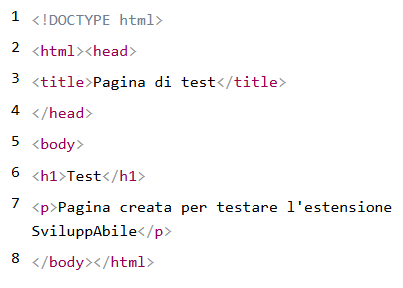
\includegraphics[width=0.5\linewidth, alt={Pagina \acrshort{html} base per effettuare i test della modalità guidata}]{img/test_MG.png}
    \caption{Pagina HTML base per effettuare i test della modalità guidata}\label{fig:pagina_test}
\end{figure}

\subsubsection*{\texttt{Come si crea un <head> che contenga tutti gli elementi utili per una pagina accessibile?}}
\begin{adjustwidth}{1cm}{1cm}
\noindent {\footnotesize Per creare un head accessibile, assicurati di includere i seguenti elementi:\\
1.  **Metatag Titolo (title)**: Utilizzato dal browser come titolo della finestra della pagina.\\
2.  **Metatag Descrizione (description)**: Descrive il contenuto della pagina e appare nella barra degli strumenti del browser e nei risultati dei motori di ricerca.\\
3.  **Metatag Chiave (keywords)**: Non più importante come in passato, ma puoi utilizzarla se necessario per le ricerche.\\
\\Inoltre, assicurati di utilizzare un markup semantico corretto per le sezioni della pagina. Ad esempio, puoi utilizzare `<header>`, `<nav>`, `<main>`, `<section>`, `<article>`, `footer>` in luogo di semplici div.\\
Infine, assicurati di aggiungere un elemento `alt` a tutte le immagini con una descrizione del contenuto dell'immagine.\\
\\CODICE SUGGERITO:\\
\texttt{1 <head>\\
2 <title>Pagina di test</title>\\
3 <meta charset="UTF-8">\\
4 <meta name="viewport" content="width=device-width, initial-scale=1.0">\\
5 <meta name="description" content="Pagina creata per testare l'estensione SviluppAbile">\\
6 <meta name="keywords" content="test,sviluppo accessibile">\\
7 </head>\\}}
\end{adjustwidth}


\subsubsection*{\texttt{Come posso ora creare dei paragrafi che rispettino le linee guida BEM?}}
\begin{adjustwidth}{1cm}{1cm}
\noindent {\footnotesize Per creare paragrafi in base alle linee guida BEM, puoi utilizzare la sintassi seguente:\\
1. Definisci un classico `.block\_\_element` per il contenuto del paragrafo: `class="block\_\_element"`\\
2. Utilizza `.block\_\_element--modificatore` per aggiungere modificatori: `class="block\_\_element --modificatore"`\\
In questo modo, i paragrafi saranno distinti e facili da identificare tramite la tecnica BEM.\\
\\Nota: Assicurati di sostituire `--modificatore` con il nome del modificatore effettivo nel tuo progetto.\\
\\CODICE SUGGERITO:\\
\texttt{1 <h1 class="block\_\_title">Titolo</h1>\\
2 <p class="block\_\_text --grande">Testo di esempio con un modificatore per il colore.</p>\\
3 <p class="block\_\_text --rosso">Testo di esempio con altro contenuto.</p>}\\
}
\end{adjustwidth}


\subsubsection*{\texttt{Come posso inserire immagini accessibili?}}
\begin{adjustwidth}{1cm}{1cm}
\noindent {\footnotesize Inserire immagini accessibili significa garantire che le informazioni contenute nelle immagini siano anche disponibili ai utenti con disabilità visiva. Ciò può essere fatto utilizzando l'attributo `alt` all'interno dell'elemento `<img>`.\\
In questo esempio, l'attributo `alt` contiene una descrizione breve e concisa della foto. Se il browser non è in grado di visualizzare l'immagine (ad esempio, se si utilizza un lettore schermo), la descrizione contenuta nell'attributo `alt` verrà visualizzata al posto dell'immagine.\\
Inoltre, per immagini decorative o grafici che non contengono informazioni importanti, è consigliabile utilizzare l'attributo `alt=""`, in modo da eliminare il testo alternativo dalla navigazione.\\
\\CODICE SUGGERITO:\\
\texttt{1 <img src="immagine.jpg" alt="Descrizione della foto">}
}
\end{adjustwidth}

\subsubsection*{\texttt{Come si crea una table rispettando le linee guida WCAG?}}
\begin{adjustwidth}{1cm}{1cm}
\noindent {\footnotesize Per creare una tabella accessibile secondo le linee guida WCAG, è importante fornire un'esperienza utente inclusiva e facilitare l'accessibilità a tutte le persone, in particolare alle persone con disabilità visive che utilizzano strumenti di lettura ad alta voce o tastiera. Ecco alcuni passaggi per creare una tabella accessibile:\\
1.  **Istruzioni per l'utilizzo della tabella**: fornire un'introduzione sulle informazioni presentate nella tabella e quali sono le colonne principali, aiutando gli utenti che utilizzano strumenti di lettura ad alta voce.\\
2.  **Tabella semantica con role="presentation" impostato su false**: questo ti permetterà a un assistente di lettura di comprendere il contenuto della tabella e fornirlo correttamente all'utente.\\
\\Nota che ogni elemento della tabella (celle, intestazioni) deve avere un id o un attributo aria-*, per fornire una descrizione dell'elemento e aiutare gli utenti con disabilità visive a comprendere il contenuto.\\
\\CODICE SUGGERITO:\\
\texttt{1 <table>\\
2 <caption>Esempio di tabella accessibile</caption>\\
3 <thead>\\
4 <tr role="row">\\
5 <th scope="col" id="nome">Nome</th>\\
6 <th scope="col" id="età">Età</th>\\
7 </tr>\\
8 </thead>\\
9 <tbody>\\
10 <tr role="row">\\
11 <td headers="nome">Mario Rossi</td>\\
12 <td headers="età">32 anni</td>\\
13 </tr>\\
14 <tr role="row">\\
15 <td headers="nome">Giovanni Bianchi</td>\\
16 <td headers="età">35 anni</td>\\
17 </tr>\\
18 </tbody>\\
19 </table>}
}
\end{adjustwidth}


\subsubsection*{\texttt{Come posso utilizzare gli attributi ARIA per migliorare l'accessibilità degli elementi interattivi?}}
\begin{adjustwidth}{1cm}{1cm}
\noindent {\footnotesize Gli attributi ARIA (Accessible Rich Internet Applications) sono stati sviluppati per rendere le applicazioni web accessibili a tutti, nonostante eventuali disabilità. Sono utilizzati per aggiungere funzionalità di navigazione e controllo agli elementi interattivi come i bottoni e gli elementi dropdown.\\
Per migliorare l'accessibilità degli elementi interattivi tramite ARIA, ti suggerisco di utilizzare le seguenti strategie:\\
1.  Utilizza il role di un elemento (ad esempio `button`, `menuitem`) per specificarne la funzione.\\
2.  Aggiungi gli attributi aria-label e aria-describedby per fornire una descrizione dell'elemento interattivo.\\
3.  Utilizza l'attributo aria-haspopup per indicare se un elemento è un menu o una lista.\\
\\In questo modo, l'elemento interattivo sarà più facile da navigare e controllare tramite strumenti assistivi come screen reader e mouse navigator.\\
Per ulteriori informazioni sugli attributi ARIA, ti consiglio di consultare la documentazione ufficiale dell'W3C.\\
\\CODICE SUGGERITO:\\
\texttt{1 <!DOCTYPE html>\\
2 <html><head>\\
3 <title>Pagina di test</title>\\
4 </head>\\
5 <body>\\
6 <!-- Utilizzo del role e degli attributi ARIA per il bottone -->\\
7 <button role="button" aria-label="Clicca per eseguire l'azione"> Esegui azione </button>\\
8 <!-- Utilizzo del role e degli attributi ARIA per il menu -->\\
9 <ul role="menu">\\
10 <li role="presentation">\\
11 <a href="\#" aria-label="Opzione 1" aria-haspopup="true">Opzione 1</a>\\
12 <ul role="sottomenu">\\
13 <li role="presentation"><a href="\#" aria-label="Sottopagina 1.1">Sottopagina 1.1</a></li>\\
14 <li role="presentation"><a href="\#" aria-label="Sottopagina 1.2">Sottopagina 1.2</a></li>\\
15 </ul></li></ul>\\
16 </body></html>}
}
\end{adjustwidth}
